\begin{tabular}[ht]{M{2.cm}M{2.cm}M{1.cm}M{1.cm}|M{1.cm}M{1.cm}|M{1.cm}M{1.cm}|M{1.cm}M{1.cm}}
  %\setlength\extrarowheight{2.5pt}
  \hline
  \multicolumn{2}{c}{Particles in cell $c$} &  \multicolumn{4}{c}{DCU} & \multicolumn{4}{c}{CTU} \\
   & & \multicolumn{2}{c}{$a/b=1$} & \multicolumn{2}{c}{$a/b=10$} & \multicolumn{2}{c}{$a/b=1$} & \multicolumn{2}{c}{$a/b=10$}\\
   % Particles & Position of particles in cell $c$ &  \multicolumn{2}{c}{DCU} & \multicolumn{2}{c}{DCU} \\
  \hline
  \hline
  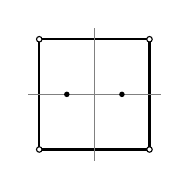
\begin{tikzpicture}[scale=0.7]
    \draw[thick] (-1.,-1.) rectangle (1.,1.);
    \draw[black!50] (-1.2,0.) -- (1.2,0.0);\draw[black!50] (.0,-1.2) -- (0.,1.2);
    %% nodes
    \fill[white] (-1,-1) circle (0.05);\draw (-1,-1) circle (0.05);
    \fill[white] (1.,-1) circle (0.05);\draw (1,-1) circle (0.05);
    \fill[white] (1,1) circle (0.05);\draw (1,1) circle (0.05);
    \fill[white] (-1.,1) circle (0.05);\draw (-1,1) circle (0.05);
    %% particles
    \fill[black] (-0.5,0.) circle (0.05);
    \fill[black] (0.5,0.) circle (0.05);
  \end{tikzpicture} & 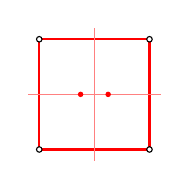
\begin{tikzpicture}[scale=0.7]
    \draw[Red,thick] (-1.,-1.) rectangle (1.,1.);
    \draw[Red!50] (-1.2,0.) -- (1.2,0.0);\draw[Red!50] (.0,-1.2) -- (0.,1.2);
    %% nodes
    \fill[white] (-1,-1) circle (0.05);\draw (-1,-1) circle (0.05);
    \fill[white] (1.,-1) circle (0.05);\draw (1,-1) circle (0.05);
    \fill[white] (1,1) circle (0.05);\draw (1,1) circle (0.05);
    \fill[white] (-1.,1) circle (0.05);\draw (-1,1) circle (0.05);
    %% particles
    \fill[Red] (-0.25,0.) circle (0.05);
    \fill[Red] (0.25,0.) circle (0.05);
  \end{tikzpicture}  &0.27 & \textcolor{Red}{0.38} & 0.41 &\textcolor{Red}{0.56} &0.29&\textcolor{Red}{0.45} &0.41& \textcolor{Red}{0.57}\\ %%% SOLUTION
  \hline
  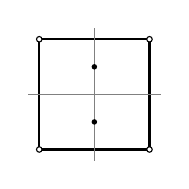
\begin{tikzpicture}[scale=0.7]
    \draw[thick] (-1.,-1.) rectangle (1.,1.);
    \draw[black!50] (-1.2,0.) -- (1.2,0.0);\draw[black!50] (.0,-1.2) -- (0.,1.2);
    %% nodes
    \fill[white] (-1,-1) circle (0.05);\draw (-1,-1) circle (0.05);
    \fill[white] (1.,-1) circle (0.05);\draw (1,-1) circle (0.05);
    \fill[white] (1,1) circle (0.05);\draw (1,1) circle (0.05);
    \fill[white] (-1.,1) circle (0.05);\draw (-1,1) circle (0.05);
    %% particles
    \fill[black] (0.,-0.5) circle (0.05);
    \fill[black] (0.,0.5) circle (0.05);
  \end{tikzpicture} & 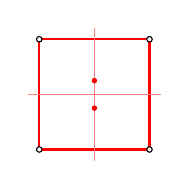
\begin{tikzpicture}[scale=0.7]
    \draw[Red,thick] (-1.,-1.) rectangle (1.,1.);
    \draw[Red!50] (-1.2,0.) -- (1.2,0.0);\draw[Red!50] (.0,-1.2) -- (0.,1.2);
    %% nodes
    \fill[white] (-1,-1) circle (0.05);\draw (-1,-1) circle (0.05);
    \fill[white] (1.,-1) circle (0.05);\draw (1,-1) circle (0.05);
    \fill[white] (1,1) circle (0.05);\draw (1,1) circle (0.05);
    \fill[white] (-1.,1) circle (0.05);\draw (-1,1) circle (0.05);
    %% particles
    \fill[Red] (0.,-0.25) circle (0.05);
    \fill[Red] (0.,0.25) circle (0.05);
  \end{tikzpicture} & 0.27 & \textcolor{Red}{0.38} & 0.54& \textcolor{Red}{0.68} & 0.29 & \textcolor{Red}{0.44} & 0.55 &\textcolor{Red}{0.71}\\ %%% SOLUTION
  \hline
  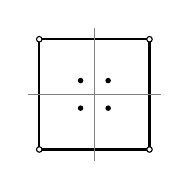
\begin{tikzpicture}[scale=0.7]
    \draw[thick] (-1.,-1.) rectangle (1.,1.);
    \draw[black!50] (-1.2,0.) -- (1.2,0.0);\draw[black!50] (.0,-1.2) -- (0.,1.2);
    %% nodes
    \fill[white] (-1,-1) circle (0.05);\draw (-1,-1) circle (0.05);
    \fill[white] (1.,-1) circle (0.05);\draw (1,-1) circle (0.05);
    \fill[white] (1,1) circle (0.05);\draw (1,1) circle (0.05);
    \fill[white] (-1.,1) circle (0.05);\draw (-1,1) circle (0.05);
    %% particles
    \fill[black] (-0.25,-0.25) circle (0.05);
    \fill[black] (0.25,-0.25) circle (0.05);
    \fill[black] (0.25,0.25) circle (0.05);
    \fill[black] (-0.25,0.25) circle (0.05);
  \end{tikzpicture}&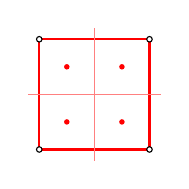
\begin{tikzpicture}[scale=0.7]
    \draw[Red,thick] (-1.,-1.) rectangle (1.,1.);
    \draw[Red!50] (-1.2,0.) -- (1.2,0.0);\draw[Red!50] (.0,-1.2) -- (0.,1.2);
    %% nodes
    \fill[white] (-1,-1) circle (0.05);\draw (-1,-1) circle (0.05);
    \fill[white] (1.,-1) circle (0.05);\draw (1,-1) circle (0.05);
    \fill[white] (1,1) circle (0.05);\draw (1,1) circle (0.05);
    \fill[white] (-1.,1) circle (0.05);\draw (-1,1) circle (0.05);
    %% particles
    \fill[Red] (-0.5,-0.5) circle (0.05);
    \fill[Red] (0.5,-0.5) circle (0.05);
    \fill[Red] (0.5,0.5) circle (0.05);
    \fill[Red] (-0.5,0.5) circle (0.05);
  \end{tikzpicture} &  0.31 &\textcolor{Red}{0.17} & 0.56 &\textcolor{Red}{0.34} & 0.33 &\textcolor{Red}{0.17} &0.57 &\textcolor{Red}{0.35} \\
  %%%%%%%%%%%%%%%%%%%%%%%%%%%%%%%%%%%%%%%
  %%%%%%%%%%%%%%%%%%%%%%%%%%%%%%%%%%%%%%% 
  \hline % Shifted left // Shifted right
  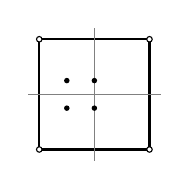
\begin{tikzpicture}[scale=0.7]
    \draw[thick] (-1.,-1.) rectangle (1.,1.);
    \draw[black!50] (-1.2,0.) -- (1.2,0.0);\draw[black!50] (.0,-1.2) -- (0.,1.2);
    %% nodes
    \fill[white] (-1,-1) circle (0.05);\draw (-1,-1) circle (0.05);
    \fill[white] (1.,-1) circle (0.05);\draw (1,-1) circle (0.05);
    \fill[white] (1,1) circle (0.05);\draw (1,1) circle (0.05);
    \fill[white] (-1.,1) circle (0.05);\draw (-1,1) circle (0.05);
    %% particles
    \fill[black] (-0.25-0.25,-0.25) circle (0.05);
    \fill[black] (0.25-0.25,-0.25) circle (0.05);
    \fill[black] (0.25-0.25,0.25) circle (0.05);
    \fill[black] (-0.25-0.25,0.25) circle (0.05);
  \end{tikzpicture} & 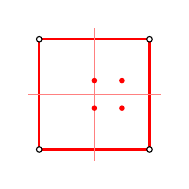
\begin{tikzpicture}[scale=0.7]
    \draw[Red,thick] (-1.,-1.) rectangle (1.,1.);
    \draw[Red!50] (-1.2,0.) -- (1.2,0.0);\draw[Red!50] (.0,-1.2) -- (0.,1.2);
    %% nodes
    \fill[white] (-1,-1) circle (0.05);\draw (-1,-1) circle (0.05);
    \fill[white] (1.,-1) circle (0.05);\draw (1,-1) circle (0.05);
    \fill[white] (1,1) circle (0.05);\draw (1,1) circle (0.05);
    \fill[white] (-1.,1) circle (0.05);\draw (-1,1) circle (0.05);
    %% particles
    \fill[Red] (-0.25+0.25,-0.25) circle (0.05);
    \fill[Red] (0.25+0.25,-0.25) circle (0.05);
    \fill[Red] (0.25+0.25,0.25) circle (0.05);
    \fill[Red] (-0.25+0.25,0.25) circle (0.05);
  \end{tikzpicture} &  0.31 &\textcolor{Red}{0.00} & 0.57 &\textcolor{Red}{0.53} & 0.34 &\textcolor{Red}{0.00} &0.58 &\textcolor{Red}{0.54}\\
  %%%%%%%%%%%%%%%%%%%%%%%%%%%%%%%%%%%%%
  %%%%%%%%%%%%%%%%%%%%%%%%%%%%%%%%%%%%%
  \hline % Shifted above // Shifted below
  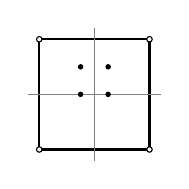
\begin{tikzpicture}[scale=0.7]
    \draw[thick] (-1.,-1.) rectangle (1.,1.);
    \draw[black!50] (-1.2,0.) -- (1.2,0.0);\draw[black!50] (.0,-1.2) -- (0.,1.2);
    %% nodes
    \fill[white] (-1,-1) circle (0.05);\draw (-1,-1) circle (0.05);
    \fill[white] (1.,-1) circle (0.05);\draw (1,-1) circle (0.05);
    \fill[white] (1,1) circle (0.05);\draw (1,1) circle (0.05);
    \fill[white] (-1.,1) circle (0.05);\draw (-1,1) circle (0.05);
    %% particles
    \fill[black] (-0.25,-0.25+0.25) circle (0.05);
    \fill[black] (0.25,-0.25+0.25) circle (0.05);
    \fill[black] (0.25,0.25+0.25) circle (0.05);
    \fill[black] (-0.25,0.25+0.25) circle (0.05);
  \end{tikzpicture} &  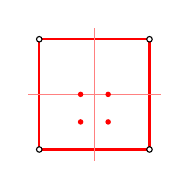
\begin{tikzpicture}[scale=0.7]
    \draw[Red,thick] (-1.,-1.) rectangle (1.,1.);
    \draw[Red!50] (-1.2,0.) -- (1.2,0.0);\draw[Red!50] (.0,-1.2) -- (0.,1.2);
    %% nodes
    \fill[white] (-1,-1) circle (0.05);\draw (-1,-1) circle (0.05);
    \fill[white] (1.,-1) circle (0.05);\draw (1,-1) circle (0.05);
    \fill[white] (1,1) circle (0.05);\draw (1,1) circle (0.05);
    \fill[white] (-1.,1) circle (0.05);\draw (-1,1) circle (0.05);
    %% particles
    \fill[Red] (-0.25,-0.25-0.25) circle (0.05);
    \fill[Red] (0.25,-0.25-0.25) circle (0.05);
    \fill[Red] (0.25,0.25-0.25) circle (0.05);
    \fill[Red] (-0.25,0.25-0.25) circle (0.05);
  \end{tikzpicture}&  0.00 &\textcolor{Red}{0.31} & 0.53 &\textcolor{Red}{0.58} & 0.00 &\textcolor{Red}{0.34} &0.54 &\textcolor{Red}{0.60} \\
  %\begin{minipage}{0.85\textwidth}\lipsum[1]\end{minipage}
\end{tabular}

%%% Local Variables: 
%%% mode: latex
%%% TeX-master: "../../mainManuscript"
%%% End: